
\begin{enumerate}
\item 
\question{There is a junction in a circuit that has one wire with current flowing in and two wires with current flowing out.  There is $1.25\myamp$ of current coming in, and the first wire going out has $0.15\myamp$ of current going out.  How much current is leaving through the second wire?}
\solution{$1.1\myamp$}
\explanation{The total amount of current leaving must equal the total amount coming in.  If we think of the unknown wire as $x$, we can say that $1.25 = x + 0.15$.  Therefore $x = 1.1\myamp$.}
\item 
\question{There is a junction in a circuit that has two wires with current flowing in and two wires with current flowing out.  The first wire with current flowing in has $0.35\myamp$ of current, the first wire with current flowing out has $0.25\myamp$ of current, and the second wire with current flowing out has $0.42\myamp$ of current.  How much current is flowing in on the second incoming wire?}
\solution{$0.32\myamp$}
\explanation{The total amount of current coming in must equal the total amount leaving.  We have two wires coming in and two wires going out.  The total going out is $0.25 + 0.42 = 0.67\myamp$.
The total coming in must equal that.  We know that one wire has $0.35\myamp$ coming in.  
Since the totals coming in must equal the total going out, we can say that $0.35 + x = 0.67$.
Therefore, our unknown wire must be $0.32\myamp$. }
\item 
\question{At a junction of four wires, wire 1 has $0.1\myamp$ of current flowing in, wire 2 has $0.2\myamp$ of current flowing in, and wire 3 has $0.4\myamp$ of current flowing out.  Is the current in wire 4 going in or out?  How much current is flowing on it?}
\solution{The current in wire 4 is going in with $0.1\myamp$ of current.}
\explanation{The total amount of current coming in must equal the total amount leaving.  Wire 1 and 2 have current coming in.  So, we can add them together and find that together they bring $0.1 + 0.2 = 0.3\myamp$ of current coming in.  Wire 4 has $0.4\myamp$ of current flowing out.  Since that is greater than the amount of current coming in, that means the last wire must have current flowing in.  The amount is $0.4 - 0.3 = 0.1\myamp$.  Therefore, wire 4 has $0.1\myamp$ of current going in.}
\item 
\question{If I have three $100\myohm$ resistors in series, what is the total resistance of the series?}
\solution{$300\myohm$}
\explanation{Resistance in series just adds together.  So we have $100 + 100 + 100 = 300\myohm$ resistance.}
\item 
\question{If I have a $10\myohm$ resistor, a $30\myohm$ resistor, and a $65\myohm$ resistor in series, what is the total resistance of the series?}
\solution{$105\myohm$}
\explanation{Resistance in series just adds together.  So we have $10 + 30 + 65 = 105\myohm$ total resistance in this series.}
\item 
\question{If I have a $5\myohm$ resistor and a $7\myohm$ resistor in series, what is the total resistance of the series?}
\solution{$12\myohm$}
\explanation{Resistance in series just adds together.  So we have $5 + 7 = 12\myohm$ resistance in this series.}
\item 
\question{If I have two resistors in parallel, a $30\myohm$ resistor and a $40\myohm$ resistor, what is the total resistance of this circuit?}
\solution{$17.14\myohm$}
\explanation{Equation~\ref{eqparallelresistancen} tells us how to add together parallel resistance:
\begin{align*}
R_T &= \frac{1}{\frac{1}{30} + \frac{1}{40}} \\
    &\approx \frac{1}{0.03333 + 0.025} \\
    &\approx \frac{1}{0.05833} \\
    &\approx 17.14 \myohm
\end{align*}
}
\item 
\question{If I have three resistors in parallel---$25\myohm$, $40\myohm$, and $75\myohm$, what is the total resistance of this circuit?}
\solution{$12.77\myohm$}
\explanation{Equation~\ref{eqparallelresistancen} tells us how to add together parallel resistance:
\begin{align*}
R_T &= \frac{1}{\frac{1}{25} + \frac{1}{40} + \frac{1}{75}} \\
    &\approx \frac{1}{0.04 + 0.025 + 0.0133} \\
    &\approx \frac{1}{0.0783}
    &\approx 12.77 \myohm
\end{align*}
}
\item 
\question{If I have four resistors in parallel---$1,000\myohm$, $800\myohm$, $2,000\myohm$, and $5,000\myohm$, what is the total resistance of this circuit?}
\solution{$338.98\myohm$}
\explanation{Equation~\ref{eqparallelresistancen} tells us how to add together parallel resistance:
\begin{align*}
R_t &= \frac{1}{\frac{1}{1,000} + \frac{1}{800} + \frac{1}{2,000} + \frac{1}{5,000}} \\
    &= \frac{1}{0.001 + 0.00125 + 0.0005 + 0.0002} \\
    &= \frac{1}{0.00295} \\
    &\approx 338.98\myohm
\end{align*}
}
\item 
\question{If I have three resistors in parallel---$100\myohm$, $5,000\myohm$, and $10,000\myohm$---what is the total resistance of this circuit?  Which of the resistors is the total resistance most similar to?}
\solution{$97.09\myohm$---this is very similar to the $100\myohm$ resistor.}
\explanation{Equation~\ref{eqparallelresistancen} tells us how to add together parallel resistance:
\begin{align*}
R_T &= \frac{1}{\frac{1}{100} + \frac{1}{5,000} + \frac{1}{10,000}} \\
    &= \frac{1}{0.01 + 0.0002 + 0.0001} \\
    &= \frac{1}{0.0103} \\
    &\approx 97.09\myohm
\end{align*}
This is very close to the $100\myohm$ resistance. 
Parallel resistance is always lower (even if slightly) than the lowest parallel resistance.
}
\item 
\question{Take a look at the following circuit diagram.  If the voltage drop between B and C is 2 volts, and the voltage drop between C and D is 3 volts, what is the voltage drop between A and E?  What is the voltage at E?  What is the voltage at A? \\ 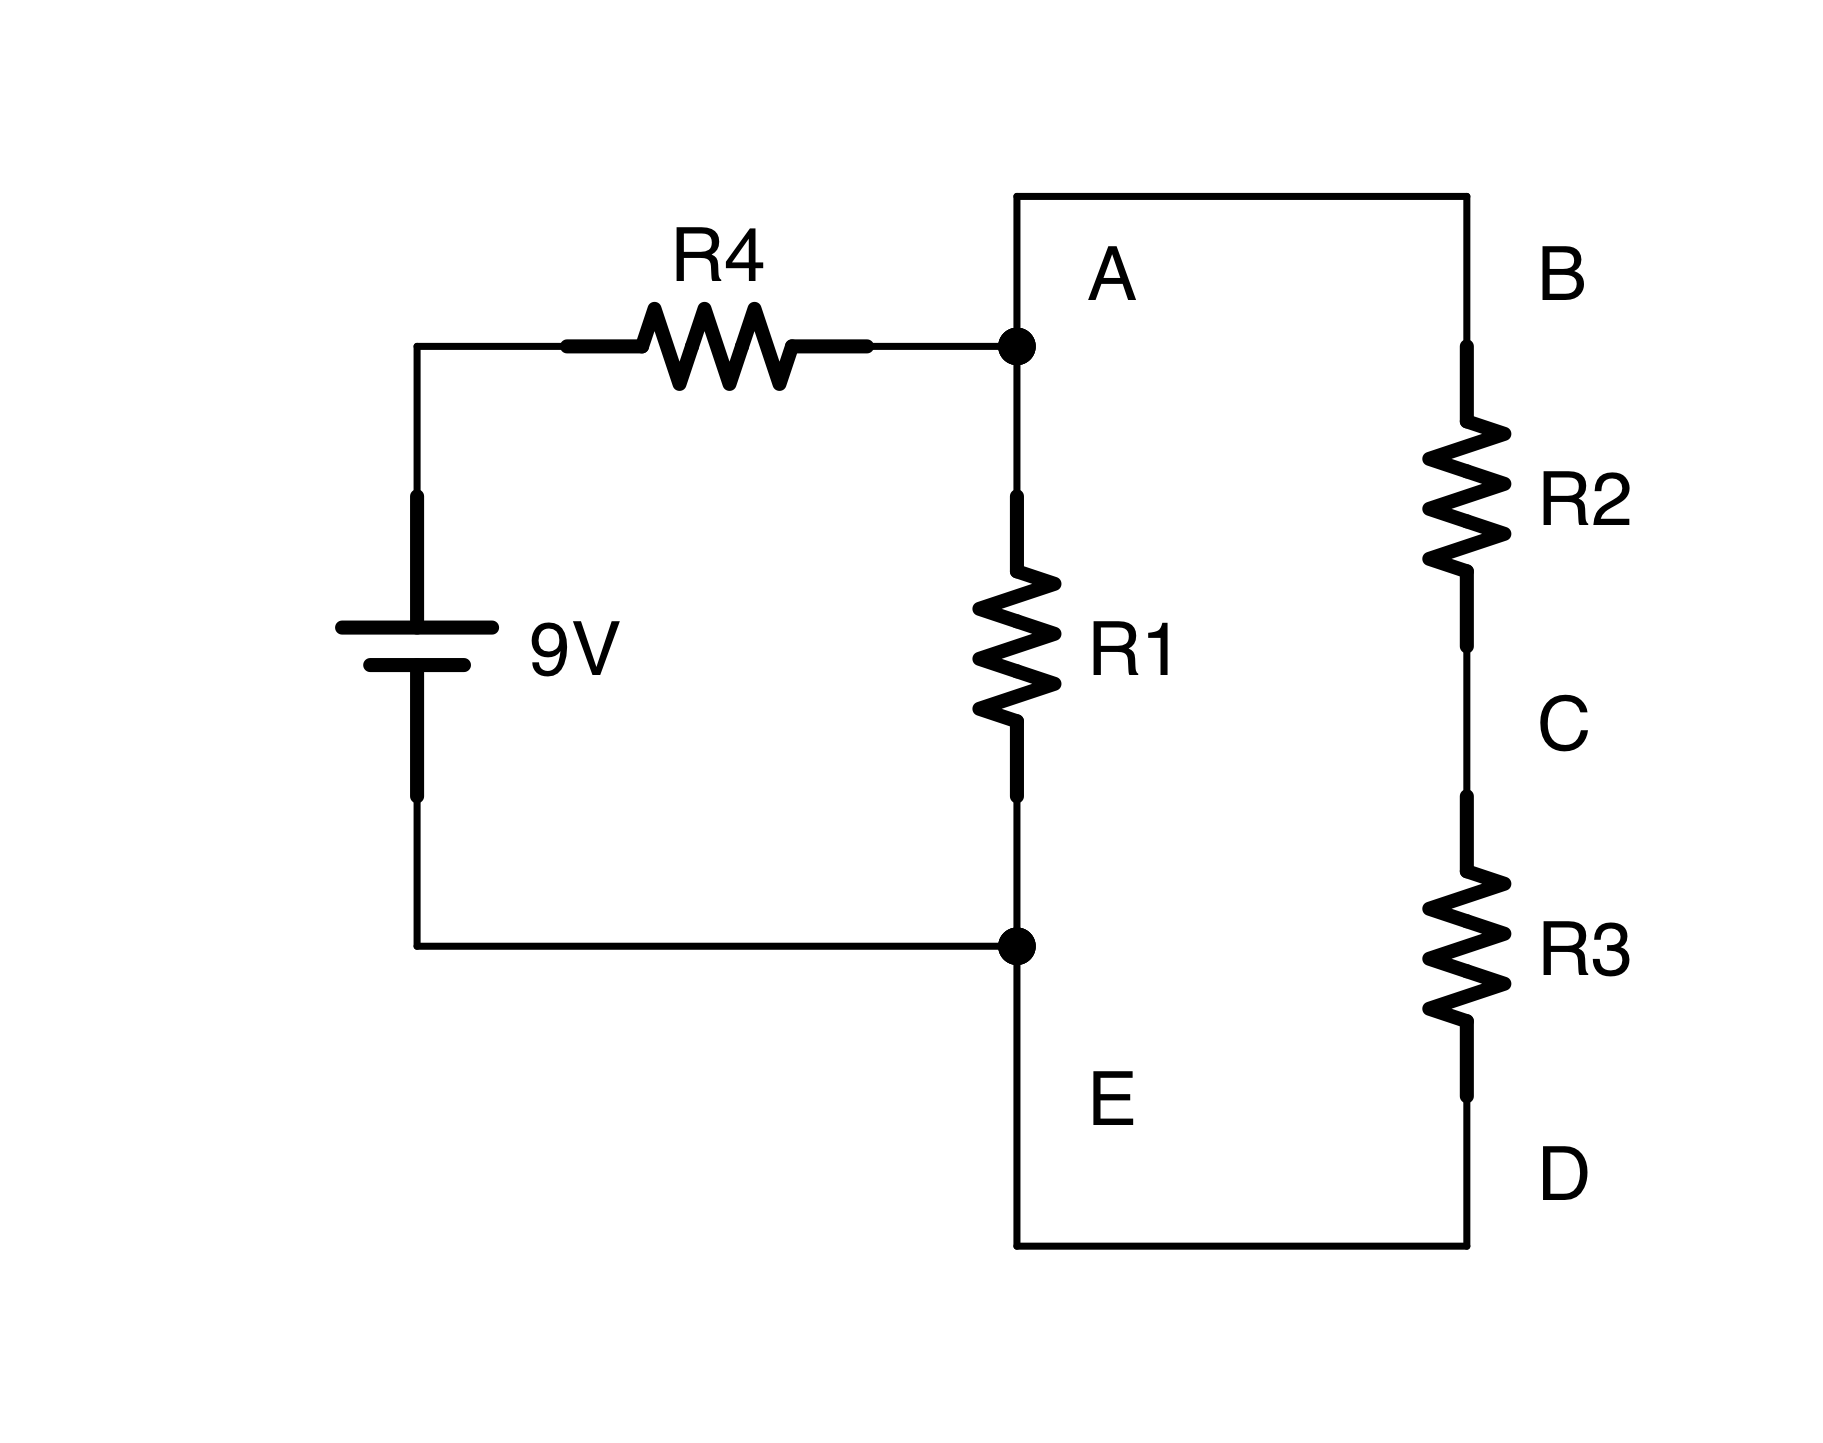
\includegraphics[scale=0.08]{VoltageDropProblem.png}}
\solution{Voltage drop between A and E is $5\myvolt$.  Voltage at E is $0\myvolt$.  Voltage at A is $5\myvolt$.}
\explanation{The voltage starts at $9\myvolt$.  
Every path from the positive of the battery to the ground must take $9\myvolt$.  
Kirchoff's Voltage Law states that every path between every two points must be the same voltage drop.
The path from A to E can take two different routes (either through R1 or through both R2 and R3) but they will \emph{both} have the same voltage drop because of Kirchoff's Voltage Law.
Therefore, since the drop across R2 is $2\myvolt$ and the drop across R3 is $3\myvolt$, the total drop is $2 + 3 = 5\myvolt$.
This is the same no matter what path you travel, so the voltage drop across R1 must also be $5\myvolt$.

So the voltage drop from A to E is $5\myvolt$.

There is no resistor between E and the ground terminal.  That means that these voltages are the same.  Therefore the voltage at E is $0\myvolt$.

Because the voltage at E is zero, the voltage at A is $5\myvolt$ above that, which is $5\myvolt$.
}
\item 
\question{If the circuit above runs with $2\myamp$ total current, what is the value of the resistor R4?}
\solution{$2\myohm$}
\explanation{Since we are imagining $2\myamp$ coming out of the battery (just to note---it is unrealistic for a battery to supply even $1\myamp$), the entire $2\myamp$ will go through resistor R4.

Now, at the end of R4, we determined that the voltage is $5\myvolt$.
Since we started with $9\myvolt$ that means that R4 had to drop us $4\myvolt$.
We can use Ohm's Law to figure out how much resistance was in that resistor:
\begin{align*}
R &= V / I \\
  &= 4 / 2 \\
  &= 2\myohm
\end{align*}
So, R4 is $2\myohm$.
}
\item 
\question{The circuit below is a combination of series and parallel resistances.  Each resistor is labelled with its resistance value, given in ohms.  Find out how much current is flowing through each resistor, and how much each resistor drops the voltage.  \\ 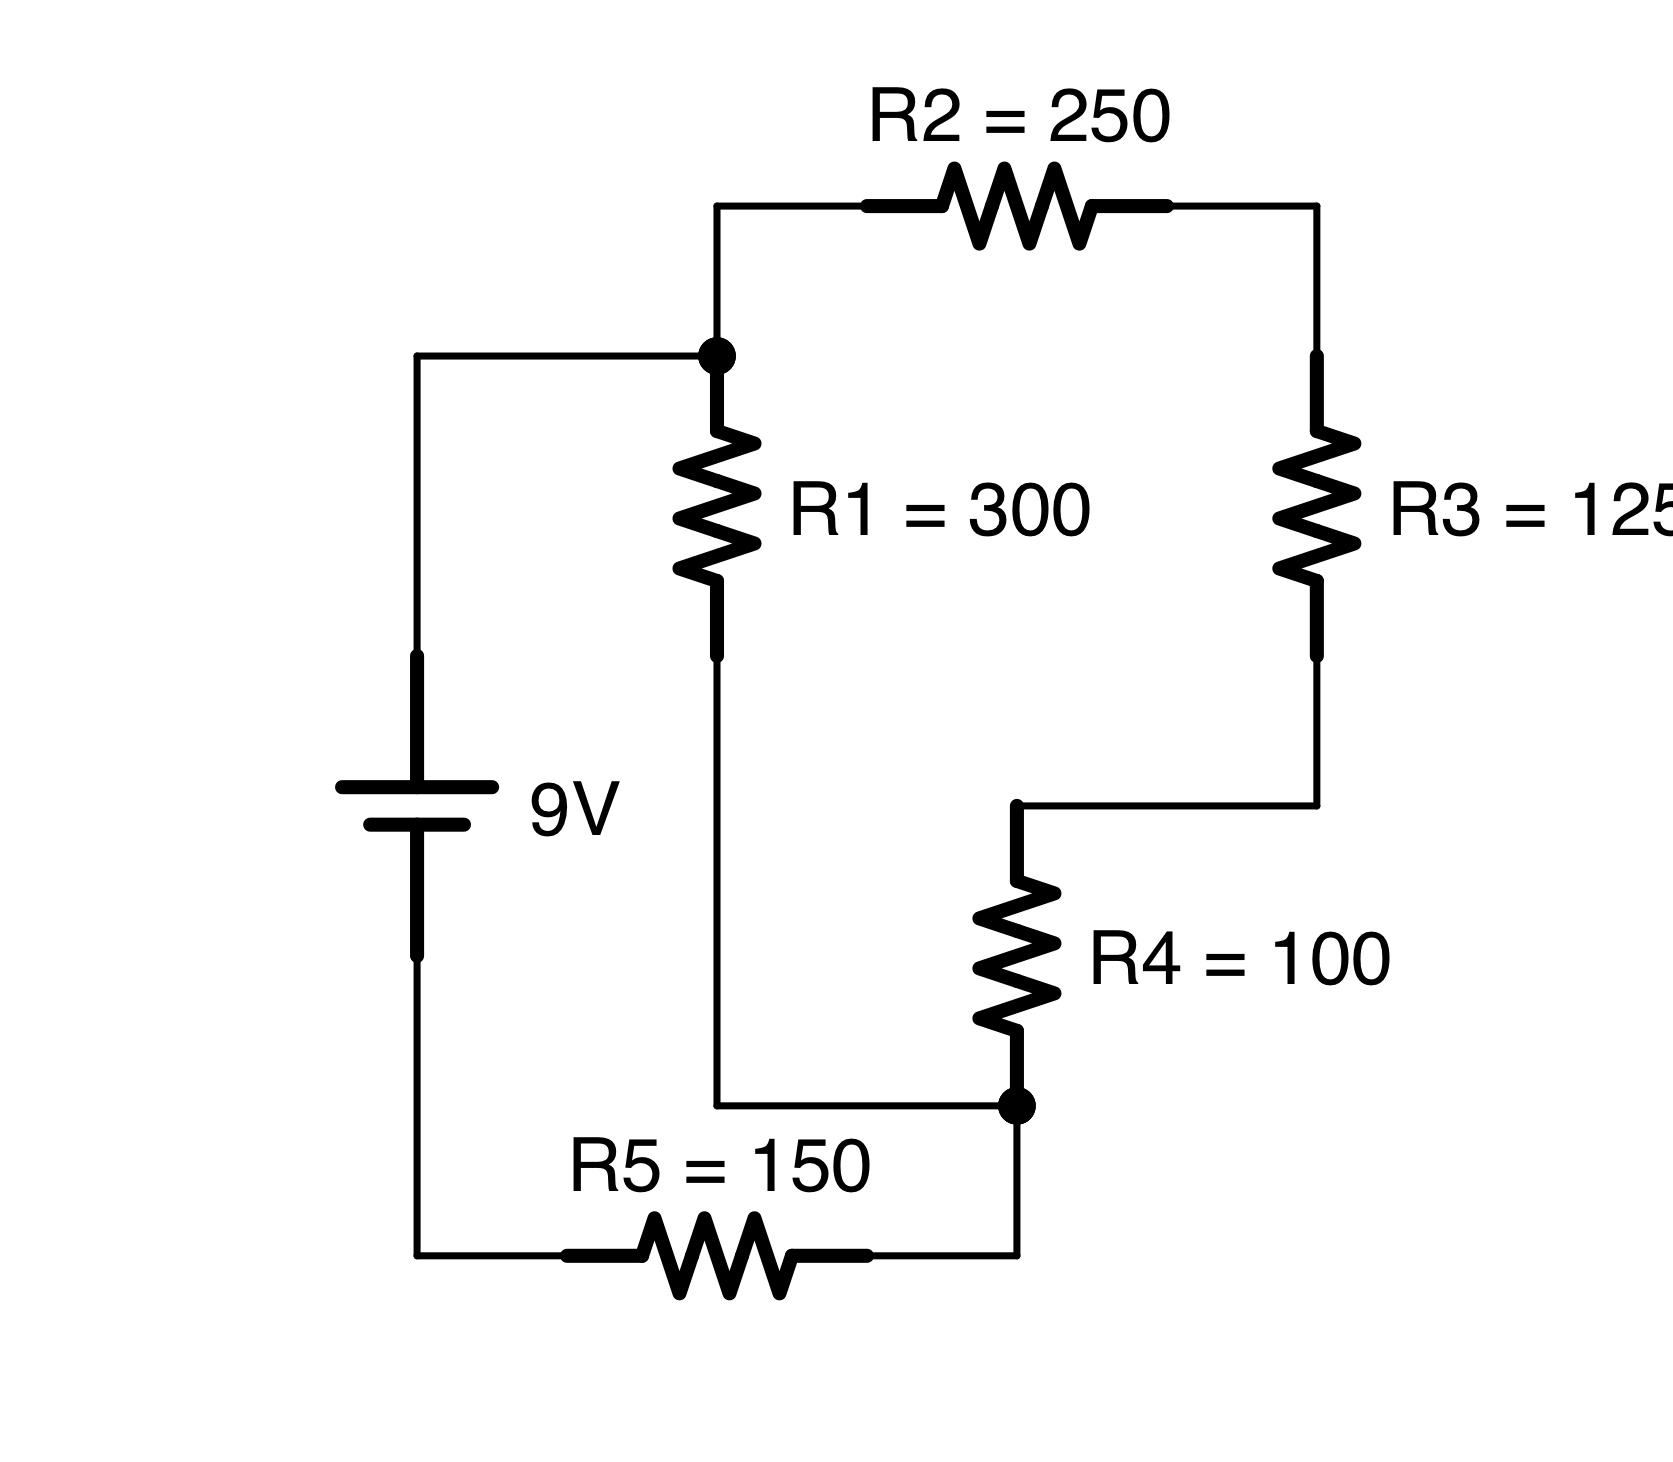
\includegraphics[scale=0.08]{ProblemCalculateCurrentAndVoltage.png}}
\solution{\begin{description}
\item[R1] $4.95\myvolt$ and $0.0165\myamp$
\item[R2] $2.625\myvolt$ and $0.0105\myamp$
\item[R3] $1.3125\myvolt$ and $0.0105\myamp$
\item[R4] $1.05\myvolt$ and $0.0105\myamp$
\item[R5] $4.05\myvolt$ and $0.025\myamp$
\end{description}
Note that these do not exactly add up correctly (because of rounding issues), but that is perfectly normal.  If you are within 1\% of the right answer, you are most likely more accurate than your equipment supports.
}
\explanation{Every circuit like this, no matter how complicated, can be solved by just breaking it down a piece at a time, and solving for each piece as you go.
The most straightforward way to solve these is to first add up \emph{all} of the resistances to get a total resistance, and then solve for total current.  
After that, you can go back through the circuit to find the individual currents and voltages.

So, the easiest way to start adding up the resistors is to take all of the resistors that are in series, and replace them with a single resistance that is the total of them.
Notice that R2, R3, and R4 are all in series with each other with no branches.
Therefore, we can replace these resistors with a single resistor that just adds up the resistances.
So, that segment has a total resistance of $250 + 125 + 100 = 475\myohm$.

That segment is in parallel with R1.
Therefore, we can use the parallel resistance rule to combine these resistances:
\begin{align*}
R_T &= \frac{1}{\frac{1}{300} + \frac{1}{475}} \\
    &\approx \frac{1}{0.00333 + 0.00211} \\
    &\approx \frac{1}{0.00544} \\
    &\approx 183.82\myohm
\end{align*}
Therefore, the whole top network---R1, R2, R3, and R4---can be replaced by a single resistance, $183.82\myohm$.
This network is in series with R5.
Therefore, we can just add these resistances together: $183.82 + 150 = 333.82\myohm$.

That's the whole resistance of the whole circuit.
We know the total voltage drop of the whole circuit, because, by definition, a $9\myvolt$ battery supplies $9\myvolt$ to the circuit.
Therefore, Ohm's Law will give us the total current:
\begin{align*}
I &= V / R \\
  &= 9 / 333.82 \\
  &= 0.0270 \myamp
\end{align*}
The battery will put out $0.027\myamp$ (i.e., $27\mymamp$) of current to this circuit.

Now we need to figure out currents and voltages to each individual component.
R5 is the easiest one to start with because it is directly connected in series with the battery terminal.
That means that all of the current will go through this resistor.
So this resistor is getting $0.027\myamp$.
We can find the voltage drop with Ohm's Law:
$$ V = I * R = 0.027 * 150 = 4.05\myvolt $$

So the current through R5 is $0.027\myamp$ and the voltage drop is $4.05\myvolt$.
That means that the voltage drop through the rest of the network is $4.95\myvolt$.
We can use that to find the currents flowing through here.

The voltage drop across R1 is $4.95\myvolt$ and the resistance is $300\myohm$.  
Therefore, the current is:
$$ I = V / R = 4.95 / 300 = 0.0165\myamp $$
Therefore, R1 has $0.0165\myamp$ flowing through it.
Since we started with $0.027\myamp$, that means the rest of the current must be flowing through the other junction.
So, the right-hand-side of the network has $0.027 - 0.0165 = 0.0105\myamp$ of current flowing through it.
Since R2, R3, and R4 are all in series, that means they all have this same current flowing through them.
To find voltages, we just use Ohm's Law:
\begin{align*}
V_{R2} &= I * R = 0.0105 * 250 = 2.625\myvolt \\
V_{R3} &= I * R = 0.0105 * 125 = 1.3125 \myvolt \\
V_{R4} &= I * R = 0.0105 * 100 = 1.05 \myvolt
\end{align*}
Note that this total voltage is actually slightly higher than what we were looking for (these add up to $4.9875\myvolt$ instead of $4.95\myvolt$ like we were expecting), but being off on the decimal point is normal when we do as much rounding as we have been.
}
\item 
\question{Build the circuit in Figure~\ref{figParallelUsingBreadboard} on your own breadboard.  Measure the voltage drops across every component, and measure the amount of current flowing into the first series resistor.}
\solution{The actual voltage drops will depend on the specific resistor values and colors of your LED.  However, in general you should have between 5 and 40 $\mymamp$ flowing through any part of your circuit.
Additionally, every complete path from positive to ground should be $9\myvolt$ (or whatever size battery you are using).}
\end{enumerate}
